\tikzstyle{reco} = [rectangle,minimum height=4em,text centered, fill=blue!20,draw=black]
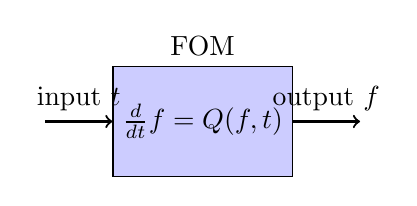
\begin{tikzpicture}[scale=0.5]
	\node [reco,label=FOM] (phys) {$\frac{d}{dt}f = Q(f,t)$};
	\draw [<-,thick] (phys)--+ (-4,0) node[midway,above] {input \(t\)};
	\draw [->,thick] (phys)--+ (4,0) node[midway,above] {output $f$};
\end{tikzpicture}
